In leading order we have to consider photon-gluon-fusion (PGF), that is
\begin{equation}
\Pggx(q) + \Pg(k_1) \rightarrow \PQ(p_1)+\PaQ(p_2)
\end{equation}
with two contributing diagrams depicted in figure \ref{fig:FeynLO}.
\begin{figure}[ht!]
\centering
\begin{subfigure}[t]{.4\textwidth}
	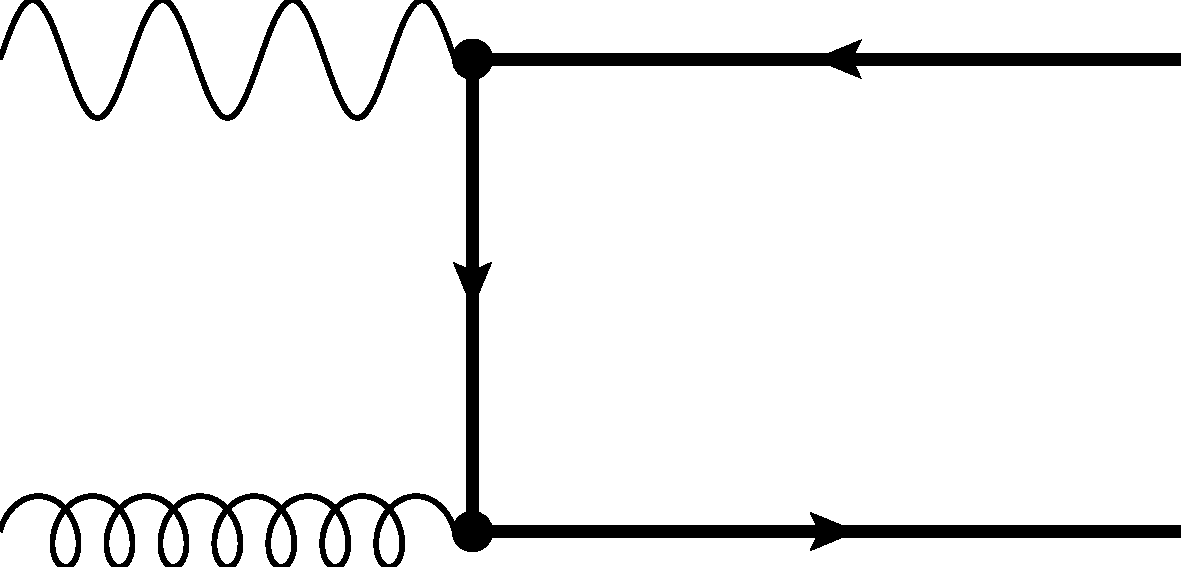
\includegraphics[width=\textwidth]{pyfeyn/lo-1}
	\caption{$i\varepsilon^{\mu}_{\Pgg}(q)\varepsilon^{\nu}_{\Pg}(k_1)\Md^{(0),1}_{\mu\nu}$}
\end{subfigure}\hspace{.15\textwidth}%
\begin{subfigure}[t]{.4\textwidth}
	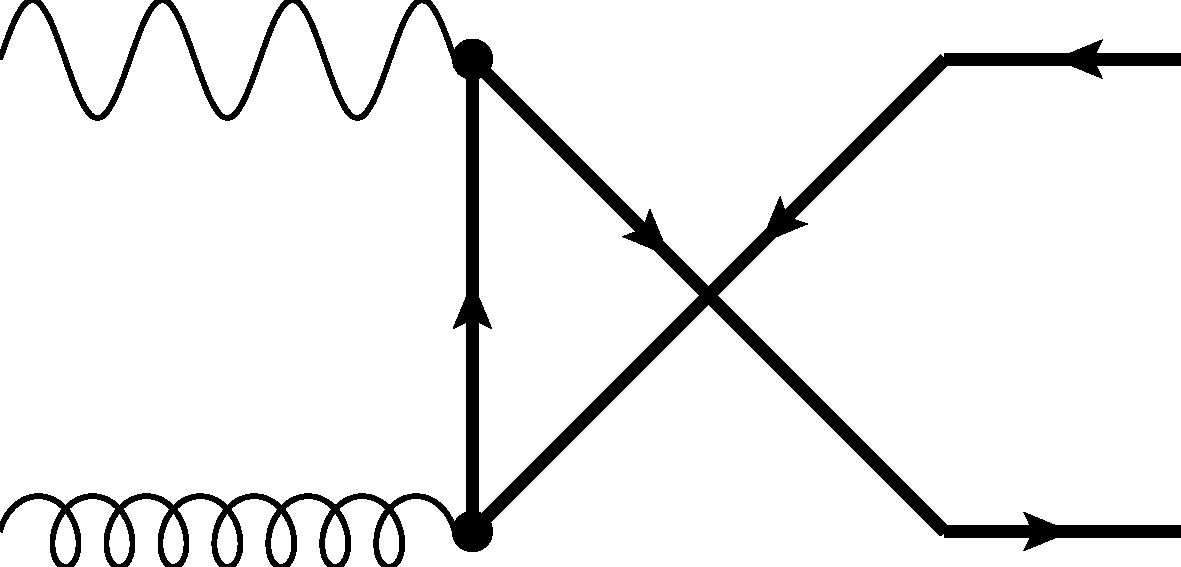
\includegraphics[width=\textwidth]{pyfeyn/lo-2}
	\caption{$i\varepsilon^{\mu}_{\Pgg}(q)\varepsilon^{\nu}_{\Pg}(k_1)\Md^{(0),2}_{\mu\nu}$}
\end{subfigure}
\caption{leading order Feynman diagrams}\label{fig:FeynLO}\fxerror{shift to appendix?}
\end{figure}

The result can then be written as
\begin{equation}
M_k^{(0)} = \hat {\mathcal P}_{k}^{\Pgg,\mu\mu'}\hat {\mathcal P}_{k}^{\Pg,\nu\nu'}\sum_{j,j'=1}^2\Md^{(0),j}_{\mu\nu}\left(\Md^{(0),j'}_{\mu'\nu'}\right)^* = 8g^2\mu_D^{-\epsilon}e^2e_H^2 N_C C_F B_{k,QED}
\end{equation}
where $g$ and $e$ are the strong and electromagnetic coupling constants respectively, $\mu_D$ is an arbitray mass parameter introduced to keep the couplings dimensionless and $e_H$ is the magnitude of the heavy quark in units of $e$. Further $N_C$ corresponds to the gauge group $SU(N_C)$ and the color factor $C_F=(N_C^2-1)/(2N_C)$ refers to the second Casimir constant of the fundamental representation for the quarks. We then find:
\begin{align}
B_{G,QED} &= \frac{t_1}{u_1} + \frac{u_1}{t_1} + \frac{4m^2s'}{t_1u_1}\left(1-\frac{m^2s'}{t_1u_1}\right)
+\frac{2s'q^2}{t_1u_1} +\frac{2q^4}{t_1u_1} + \frac{2m^2q^2}{t_1u_1}\left(2-\frac{{s'}^2}{t_1u_1}\right)\nonumber\\
 &\hspace{20pt}+\epsilon\left\{ -1 + \frac{{s'}^2}{t_1u_1} + \frac{s'q^2}{t_1u_1} -
\frac{q^4}{t_1u_1} - \frac{m^2q^2{s'}^2}{t_1^2u_1^2} \right\} + \epsilon^2\frac{{s'}^2}{4t_1u_1}\\
B_{L,QED} &= -\frac{4q^2}{s'}\left(\frac s {s'} - \frac{m^2s'}{t_1u_1}\right)\\
B_{P,QED} &= \frac 1 2\left(\frac{t_1}{u_1}+\frac{u_1}{t_1}\right)\left(\frac{2m^2 s'}{t_1u_1}-1 - \frac{2q^2}{s'}\right)\\
B_{k,QED} &= B^{(0)}_{k,QED} + \epsilon B^{(1)}_{k,QED} + \epsilon^2 B^{(2)}_{k,QED}
\end{align}

By using eq. (\ref{eq:PartonicStructureTensor0}) we can derive the $n$-dimensional $2\rightarrow 2$ phase space
\begin{equation}
dPS_2 = \!\int\!\!\frac{d^{n}p_1}{(2\pi)^{n-1}}\frac{d^{n}p_2}{(2\pi)^{n-1}}\Theta(p_{1,0})\delta(p_1^2-m^2)\Theta(p_{2,0})\delta(p_2^2-m^2)(2\pi)^n\delta^{(n)}(k_1+q-p_1-p_2)
\end{equation}
that can be solved by using the center-of-mass system (CMS) of the incoming particles\cite{Bojak:2000eu}
\begin{align}
q &= \left(\frac {s+q^2}{2\sqrt s},0,0,-\frac{s-q^2}{2\sqrt s},\hat 0\right) &
k_1 &= \frac {s-q^2}{2\sqrt s}\left(1,0,0,1,\hat 0\right)
\end{align}
such that $q+k_1=(\sqrt s,\vec 0)$ and $k_1^2 = 0$. For the outgoing particles it follows
\begin{align}
p_1 &= \frac{\sqrt s} 2 \left(1,0,-\beta\sin\theta_1,-\beta\cos\theta_1,\hat 0\right)&
p_2 &= \frac{\sqrt s} 2 \left(1,0,\beta\sin\theta_1,\beta\cos\theta_1,\hat 0\right)
\end{align}
such that $p_1+p_2 = (\sqrt s,\vec 0)$ and $p_1^2 = p_2^2=m^2$ and 
\begin{equation}t_1 = -\frac{s'}{2}(1-\beta \cos(\theta_1)), \quad u_1=-\frac{s'}{2}(1+\beta \cos(\theta_1))\end{equation}

We then arrive at the well known result\cite{Harris:1995tu}:
\begin{align}
dPS_2 &= \frac{\beta \sin(\theta_1)}{16\pi\Gamma(1+\epsilon/2)}\left(\frac{s\beta^2\sin^2(\theta_1)}{16\pi}\right)^{\epsilon/2}d\theta_1
\end{align}

The cross sections are then given by:
\begin{align}
d\sigma_k^{(0)} = \frac{1}{2s}\frac {K_{\Pgg\Pg} E_k(\epsilon)} 2 b_k(\epsilon) M_k^{(0)} dPS_2
\end{align}

The procedure is completely analogous to the inclusive case \cite{Laenen1993162}\fxerror{add my cite} and the results agree.
